\documentclass[12pt]{article}
\usepackage{epsfig, amsmath, amssymb}
\newcommand{\pfdotx}{\vec{p}_f \cdot \vec{x}}
\newcommand{\pfdotz}{\vec{p}_f \cdot \vec{z}}
\newcommand{\qdoty}{\vec{q} \cdot \vec{y}}
\begin{document}
\hfill \today\\[1.0ex]
\noindent {\Large\bfseries Construction of 3pt.\ Meson Correlators with sequential source}\\[1.0ex]

\section{Construction of Euclidean Three-point Function}

A connected three-point function in Euclidean space-time can be written
\begin{equation}
\tilde{\Gamma}(t_f, t; \vec{p}_f, \vec{q}) = \sum_{\vec{x},
\vec{y}} e^{-i\pfdotx}
e^{+i\vec{q}\cdot\vec{y}} \; \Big\langle 0 \Big| \bar{d}\Gamma_f u(\vec{x}, t_f) \cdot \bar{u} \Gamma u(\vec{y}, t) \cdot \bar{u} \Gamma_i d(\vec{0}, 0) \Big| 0 \Big\rangle ,
\end{equation}
where we are considering the current insertion to be on the quark labelled
$u$.
\vspace{-4cm}
\begin{figure}[!h]
\begin{center}
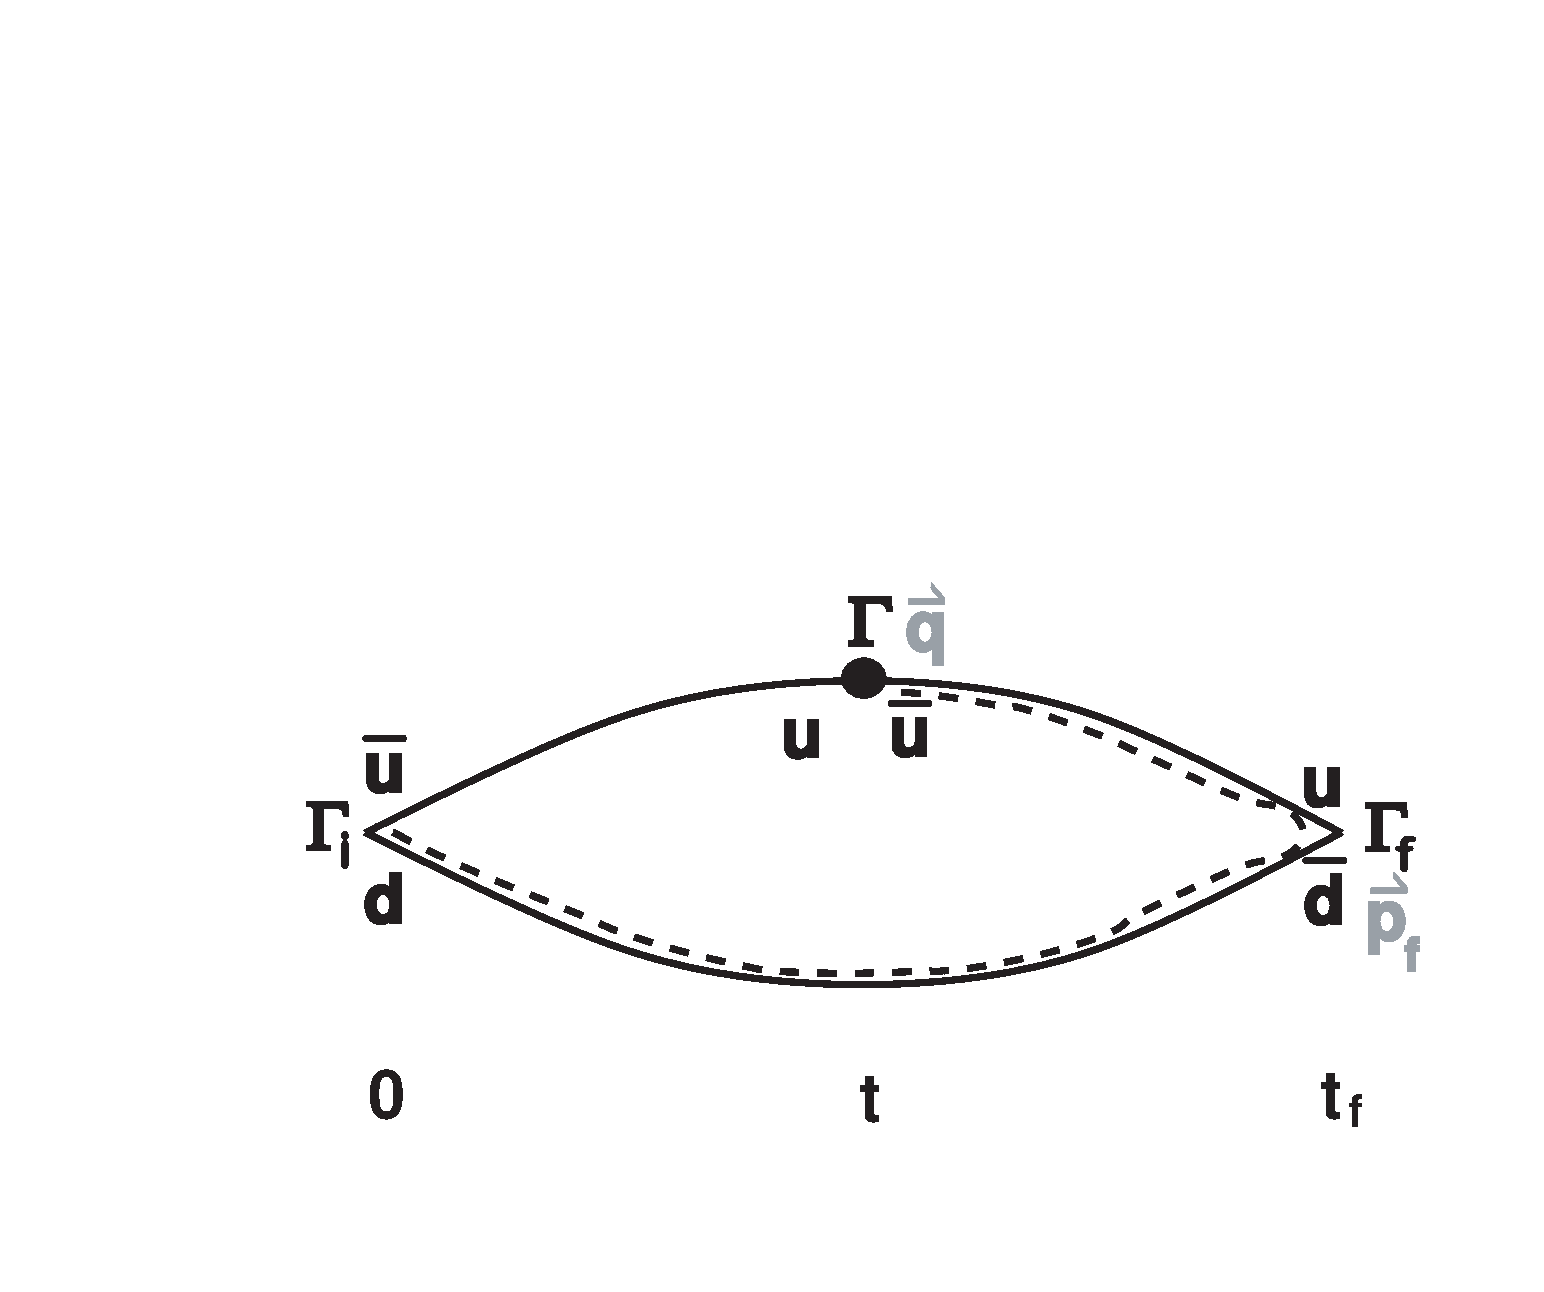
\psfig{width=11cm,file=three_point.eps}
\caption{The dotted line shows the sequential-source
  propagator computed in the calculation.}
\end{center}
\end{figure}

Introducing the quark propagators for the $u$ and $d$ quarks as
follows
\begin{eqnarray}
U^{ij}_{\alpha\beta} (x,y) & = & \langle u^i_{\alpha}(x)
\bar{u}^j_{\beta}(y)\rangle\\
D^{ij}_{\alpha\beta} (x,y) & = & \langle d^i_{\alpha}(x)
\bar{d}^j_{\beta}(y)\rangle,
\end{eqnarray}
we can write the appropriate Wick contraction as
\begin{equation} \label{eq:u_quark_3pt}
\tilde{\Gamma}(t_f, t; \vec{p}_f, \vec{q}) = - \sum_{\vec{x},
\vec{y}} e^{-i\pfdotx}
e^{+i\vec{q}\cdot\vec{y}} \;   \mathrm{tr} \Big\langle D(0,x)\, \Gamma_f\, U(x,y)\, \Gamma\, U(y,0)\, \Gamma_i  \Big\rangle ,
\end{equation}
where it will turn out that $\vec{q}=\vec{p}_f - \vec{p}_i$.

{\bf N.B. Chroma output is the trace, i.e.} $- \tilde{\Gamma}(t_f, t; \vec{p}_f, \vec{q})$.




\section{Sequential-Source Propagators}
There are two ways of expressing the three-point correlators in terms
of sequential-source (or extended, or exponentiated) propagators.  In
the first method, we compute the sequential propagator with the
\textit{operator} as the sequential source; this method has the
advantage of allowing the matrix elements of a particular operator, at
a particular momentum, to be evaluated for \textit{any} external
states.  The second method employs the final hadron state as the
sequential source.  This method in general allows \textit{any} current
insertion to be evaluated for only \textit{particular} final and, in
the case of baryons, initial states, and is the method we are using in
this calculation.

\subsection{Lattice quark propagators.}
The general quark propagator
\begin{equation}
G^{ij}_{\alpha\beta}(x,y) = \langle q^i_{\alpha}(x)
\bar{q}^j_{\beta}(y)\rangle
\end{equation}
satisfies
\begin{equation}
M^{ik}_{\alpha\gamma}(x,z) G^{kj}_{\gamma\beta}(z,y) = \delta_{ij}
\delta_{\alpha \beta} \delta_{xy}\label{eq:dirac_eqn}
\end{equation}
where $M$ is the lattice Dirac operator.  The anti-quark propagator
is related through
\begin{equation}
G(y,x) = \gamma_5 G(x,y)^{\dagger} \gamma_5,\label{eq:anti_quark}
\end{equation}
which is a simple property of the lattice Dirac equation.
\textit{Note}: it is important to check for consistency in the
normalisation of the quark propagators.

\subsection{Sequential-source propagator for $u$ insertion.}
Chroma computes the following extended propagator, given the already
computed ``forward'' propagator $F=G(y,0)=D(y,0)=U(y,0)$,
\begin{equation}
H_{\Gamma_f}(y,0; t_f; \vec{p}_f) \equiv \sum_{\vec{x}} e^{i \pfdotx} U(y,x) \gamma_5 \Gamma_f^\dag \gamma_5 D(x,0) \gamma_5\label{eq:u_insert}
\end{equation}
for the case of degenerate quark masses, i.e.\ equivalent $u$- and
$d$-quark propagators, and for a specified $\vec{p}_f$ and $t_f$.  Using
the Dirac equation, eqn.~\ref{eq:dirac_eqn}, we see that
\begin{equation}
M(z,y) H_{\Gamma_f}(y,0; t_f; \vec{p}_f) = \delta_{t_z, t_f} e^{i
  \pfdotz} \gamma_5 \Gamma_f^\dag \gamma_5 D(z,0) \gamma_5,
  \label{eq:dirac_u_insert}
\end{equation}
where the RHS will serve as the source for the inversion that yields
$H_{\Gamma_f}$.

Taking the complex conjugate of eqn.~\ref{eq:u_insert}, we have 
\begin{eqnarray}
H_{\Gamma_f} (y,0; t_f; \vec{p}_f)^{\dagger} & = & \sum e^{-i\pfdotx}\gamma_5
D^{\dagger}(x,0)\gamma_5 \Gamma_f \gamma_5  U^{\dagger}(y,x)\nonumber\\
& = & \sum e^{-i\pfdotx} D(0,x) \Gamma_f U(x,y) \gamma_5,
\end{eqnarray}
using eqn.~\ref{eq:anti_quark}. The hanging $\gamma_5$ is a ``fake'' pion source used in the code - we'll discuss it further later. Finally, comparing with
eqn.~\ref{eq:u_quark_3pt}, inserting a $(\gamma_5)^2 =1 $ and using the cyclic property of the trace,
we see that
\begin{equation}
\tilde{\Gamma}(t_f, t; \vec{p}_f, \vec{q}) = - \sum_{\vec{y}} e^{+i\vec{q}\cdot\vec{y}} \;   \mathrm{tr} \Big\langle \gamma_5 H_{\Gamma_f}^\dag(y, 0; t_f; \vec{p}_f) \gamma_5  \, \Gamma\, U(y,0)\, \Gamma_i \gamma_5  \Big\rangle ,
\label{eq:u_quark_3pt_final}
\end{equation}

\subsection{Chroma code}

mesonseqsrc\_w.cc is called by hadseqsrc\_w.cc and returns an object  $F^\dag \gamma_5 \Gamma_f$ for a supplied forward propagator $F$.
\begin{verbatim}
00071   LatticePropagator mesPionXSeqSrc(const multi1d<LatticePropagator>
                                & quark_propagators,
00072                                    int insertion)
...
00091     fin = adj(quark_propagators[0]) * Gamma(G5) * Gamma(insertion);
\end{verbatim}
In hadseqsrc\_w.cc this object is acted on to return the source we seek for $H_{\Gamma_f}$, $\delta_{t_z, t_f} e^{i
  \pfdotz} \gamma_5 \Gamma_f^\dag \gamma_5 D(z,0) \gamma_5 $, if $D(z,0)$ is supplied as $F$.
\begin{verbatim}
00061     /* Now take hermitian conjugate and multiply on both sides
00062        with gamma_5 = Gamma(15) */
00063     {
00064       /* This bit does the hermitian conjugation. */
00065       LatticePropagator q1_tmp = adj(src_prop_tmp);
00066       src_prop_tmp = q1_tmp;
00067     }
...
00072     {
00073       /* Now slap the gamma_5 on either end */
00074       LatticePropagator q1_tmp = src_prop_tmp * Gamma(15);
00075       src_prop_tmp = Gamma(15) * q1_tmp;
\end{verbatim}

In inline\_building\_blocks\_w.cc a table describes what is meant by the ``backward'' propagator. Our formulae correcpond to the choice ``G5\_B\_G5''.
\begin{verbatim}
00490       //#####################################//
00491       // Convert Backward Propagator Format                      //
00492        //#####################################//
00493     
00494       if( params.bb.BkwdProps[loop].BkwdPropG5Format == "G5_B" )
00495       {
00496         LatticePropagator Bu = B[0];
00497         B[0] = Gamma( 15 ) * Bu;
00498       }
00499       else if( params.bb.BkwdProps[loop].BkwdPropG5Format == "B_G5" )
00500       {
00501         LatticePropagator Bu = B[0];
00502         B[0] = Bu * Gamma( 15 );
00503       }
00504       else if( params.bb.BkwdProps[loop].BkwdPropG5Format == "G5_B_G5" )
00505       {
00506         LatticePropagator Bu = B[0];
00507         B[0] = Gamma( 15 ) * Bu * Gamma( 15 );
00508       }
\end{verbatim}

With this choice BuildingBlocks\_w.cc is evaluating \ref{eq:u_quark_3pt_final}:
\begin{verbatim}
00145     //LatticeComplex Trace = trace( adj( B ) * 
                           Gamma( i ) * F * Gamma( GammaInsertion ) );
\end{verbatim}
where $B^\dag = \gamma_5 H_{\Gamma_f}^\dag \gamma_5$, $\Gamma(i)$ is
the current insertion, which is looped over, $F= U(y,0)$, and
$\Gamma(\mathrm{ins.})=\Gamma_i \gamma_5$. The ``insertion'' choices
are supplied as a list and should such that when right multiplied by
$\gamma_5$ they give the correct source interpolator [this is because
in mesonseqsrc the source is always assumed to be a pion, i.e. an
extra $\gamma_5$ is being carried through]. The document
``chroma\_gamma\_matrices'' lists the appropriate correections.

%\section{Relation to matrix elements}

%This is most easily done by constructing the Minkowski three-point
%function and finding the mapping to the Euclidean version. We'll take
%as a concrete example the pion form-factor, defined by
%\begin{equation}\label{}
%  \langle \pi(\vec{p}') | V^\mu(0) | \pi(\vec{p})\rangle = f(Q^2) (p'+p)^\mu,
%\end{equation}
%where $f(Q^2)$ can be shown to be real by time-reversal invariance. We
%can define a Minkowski three-point function using hermitian
%interpolating fields by
%\begin{equation}\label{}
%  \Gamma^\mu(t_f, t; \vec{p}_f, \vec{q}) = \sum_{\vec{x},
%\vec{y}} e^{-i\pfdotx} e^{+i\vec{q}\cdot\vec{y}} \; \Big\langle 0 \Big| \bar{\psi}i\gamma^5 \psi(\vec{x}, t_f) \cdot \bar{\psi} \gamma^\mu \psi(\vec{y}, t) \cdot \big( \bar{\psi} i\gamma^5 \psi(\vec{0}, 0) \big)^\dag \Big| 0 \Big\rangle 
%\end{equation}
%where we are imagining Wick contracting as before and where the dagger
%on the final factor does nothing since it is hermitian.












%\subsection{Sequential-source propagator for $d$ insertion.}
%This is computed the same way, with the r\^{o}les
%of the $U$ and $D$ reversed, so that
%\begin{equation}
%H^d (y,0; t_f, \vec{p}) = \sum_{\vec{x}} e^{i \pdotx} D(y,x) \gamma_5
%U(x,0) \gamma_5\label{eq:d_insert}
%\end{equation}
%whence
%\begin{equation}
%H^d (y,0; t_f, \vec{p})^{\dagger} = \sum e^{-i\pdotx}\gamma_5
%U^{\dagger}(x,0)\gamma_5 D^{\dagger}(y,x)
%\end{equation}

%To see how we now construct the $d$-quark insertion in the propagator,
%we now take the conjugate of eqn.~\ref{eq:d_quark_3pt}
%\begin{eqnarray}
%\Gamma_{\pi^+ \mu \pi^+}^D(t_f, t; \vec{p},\vec{q})^*  & =  & e_d
%  \sum_{\vec{x},\vec{y}} e^{+i \pdotx + i \vec{q}\cdot\vec{y}} {\rm
%  Tr} \left\{ \gamma_{\mu} D(0,y)^{\dagger} \gamma_5 U(x,0)^{\dagger}
%  \gamma_5 D(y,x)^{\dagger}
%  \right\}.\nonumber\\
%& = & e_d \sum_{\vec{y}} e^{i\qdoty} {\rm Tr} \left\{ \gamma_{\mu}
%  D(0,y)^{\dagger}  H^d(y,0; t_f, -\vec{p})^{\dagger}
%  \right\}\nonumber\\
%& = & - e_d \sum_{\vec{y}} e^{i\qdoty} {\rm Tr} \left\{ H^d(y,0;t_f,
%  -\vec{p})^{\dagger} \gamma_5 \gamma_{\mu}
%  D(y,0) \gamma_5 \right\}
%\label{eq:d_quark_3pt_final}
%\end{eqnarray}

%Comparing eqns.~\ref{eq:u_quark_3pt_final} and
%\ref{eq:d_quark_3pt_final}, we see that they are both of the same form
%and involve only propagators computed in the SZIN code.  Finally, for
%the case where $m_d = m_u \equiv m_q$, we see that both expressions
%are essentially the same, and in particular
%\begin{eqnarray}
%\lefteqn{\sum_{\vec{y}} e^{i\qdoty} {\rm Tr} \left\{ H(y,0;t_f,
%  \vec{p})^{\dagger} \gamma_5 \gamma_{\mu}
%  Q(y,0) \gamma_5 \right\}\qquad  } \nonumber \\
%   & = & \frac{1}{e_u} \Gamma^U_{\pi^+ \mu
%  \pi^+}(t_f, t; \vec{p}, \vec{q})\nonumber \\ 
%  & = & - \frac{1}{e_d} \Gamma^D_{\pi^+ \mu
%  \pi^+}(t_f, t; - \vec{p}, - \vec{q})^*
%\end{eqnarray}

%\section{Calculation of $\rho \longrightarrow \pi$ transition form factors}

%This form factor we can essentially get for free from the propagators
%computed for the pion form factor.  UKQCD has a lot of experience in
%doing this, in particular for the $B \longrightarrow \rho l \bar{\nu}$
%transitions, so I have essentially just translated the UKQCD calculation to
%the light-quark sector\cite{ukqcd95}

%\subsection{Form Factor Definitions}
%There is a single vector and three axial-vector transition form
%factors:
%\begin{eqnarray}
%\langle \pi | (V_{\mu} - A_{\mu}) | \rho \rangle & = & T_{\mu\beta}
%\epsilon_r^{\beta}\\
%T_{\mu\beta} & = & \frac{2V(q^2)}{m_\pi + m_{\rho}}
%\epsilon_{\mu\gamma\delta\beta} p^{\gamma}_{\pi} p^{\delta}_{\rho} + i
%(m_{\pi} + m_{\rho}) A_1(q^2) g_{\mu\beta}+ \nonumber \\
%& & i \frac{A_2(q^2)}{m_\pi + m_{\rho}}(p_\pi + \_\rho)_{\mu}
%q_{\beta} + i \frac{A(q^2)}{q^2} 2 m_{\rho} q_{\mu} (p_\pi +
%p_{\rho})_{\beta},
%\end{eqnarray}
%where $q = p^\pi - p^\rho$, $\epsilon$ is the $\rho$ polarisation
%vector, and $r$ is the polarisation label.  There are several
%competing definitions of the form factors, but we can postpone that
%discussion until later.

%\subsection{Two-point Functions}
%The two-point function for the pion comes straight from the pion form
%factor analysis that Randy has described:
%\begin{eqnarray}
%\Gamma_{\pi^+ \pi^+}(t_f; \vec{p}) & = & \sum_{\vec{x}} \langle
%\phi_{\pi}(\vec{x}, t_f) \phi_{\pi}^{\dagger} (0) \rangle e^{- i
%\vec{p}\cdot x}\\ & \longrightarrow & \frac{1}{2 E_{\pi}(\vec{p})}
%|Z_P(|\vec{p}_{\pi}|)|^2 e^{- E_{\pi}(\vec{p}) t_f}.
%\end{eqnarray}
%In the case of the $\rho$ meson, we introducting the interpolating
%operator
%\begin{eqnarray}
%\Omega_{\mu} & = & \bar{d} \gamma_\mu u \nonumber \\
%\Omega_{\mu}^{\dagger} & = & \Delta_\mu \bar{u} \gamma_\mu d
%\end{eqnarray}
%where $\Delta_i = -1 (i = 1,2,3)$ and $\Delta_4 = +1$,
%and determine the correlation function
%\begin{equation}
%\Gamma_{\rho^+ \rho^+, ij}(t_f, \vec{p}) = \sum_{\vec{x}} \langle
%\Omega_i(\vec{x}, t_f) \Omega_j(0)^{\dagger} \rangle e^{-i\pdotx}.\label{eq:rho_2pt}
%\end{equation}
%{\cal N.B.} at non-zero momentum, the temporal component $\Omega_0$
%also has an overlap with the vector meson; in principle we could use
%it also, but I would be worried about the effect of smearing.

%We define the overlap of the $\rho$ interpolating operator through
%\begin{equation}
%\langle 0 \mid \Omega_i(0) \mid \rho, r,\vec{p} \rangle = Z_V(|\vec{p}|)
%\epsilon_i^r
%\end{equation}
%where $r$ is the polarization index.  I have always assumed, though
%this should be checked, that this expression carries through
%straightforwardly to the case of smeared interpolating operators, with
%the complication that the overlap $Z_V$ depends on the spatial
%momentum.  The polarization vectors satisfy
%\begin{equation}
%\sum_{r = 1,2} \epsilon_i^r(\vec{p}) \epsilon_j^r(\vec{p}) = \left(-
%  g_{ij} + \frac{p_i p_j}{m_{\rho}^2}\right).
%\end{equation}
%Inserting into the correlator eqn.~\ref{eq:rho_2pt}, we have
%\begin{eqnarray}
%  \lefteqn{\Gamma_{\rho^+ \rho^+, ij}(t_f, \vec{p}) = } &  &\nonumber\\
%&  & \sum_{N,r,\vec{k}}
%\sum_{\vec{x}} \frac{1}{(2\pi)^3} \frac{1}{2 E_N(\vec{k})} \langle 0 |
%\Omega_i(\vec{x}, t_f) | N,r,\vec{k} \rangle \langle N,r,\vec{k} |
%\Omega_j(0)^{\dagger}|0 \rangle e^{-i\pdotx}.\nonumber\\
%& = & \sum_{N,r,\vec{k}}
%\sum_{\vec{x}} \frac{1}{(2\pi)^3} \frac{1}{2 E_N(\vec{k})} \langle 0 |
%\Omega_i(0) | N,r,\vec{k} \rangle \langle N,r,\vec{k} |
%\Omega_j(0)^{\dagger}|0 \rangle e^{-i\pdotx +i \vec{k}\cdot\vec{x} - i
%E_N(\vec{k}) t_f}.\nonumber\\
%& \longrightarrow & \sum_r \langle 0 |
%\Omega_i | N,r,\vec{p} \rangle \langle N,r,\vec{p} |
%\Omega_j^{\dagger}|0 \rangle e^{-i E_{\rho}(\vec{p}) t} + \mbox{higher
%  terms}\nonumber \\
%& = & \frac{1}{2 E_\rho(\vec{p})} \left( -\delta_{ij} + \frac{p_i
%    p_j}{m_{\rho}^2} \right) |Z_V(|\vec{p}|)|^2 e^{-i E_{\rho}(\vec{p}
%    )t_f}
%\end{eqnarray}
%Finally, summing over the spatial indices we have
%\begin{equation}
%\Gamma_{\rho^+ \rho^+}(t_f, \vec{p}) \equiv \sum_i \Gamma_{\rho^+
%  \rho^+, ii}(t_f, \vec{p}) = -\frac{1}{2 E_{\rho}(\vec{p})} \left( 3 -
%  \frac{\vec{p}^2}{m_{\rho}^2} \right) |Z_V(|\vec{p}|)|^2 e^{-i
%  E_{\rho}(\vec{p}) t_f }
%\end{equation}

%\subsection{Three-point Functions}
%We begin by considering
%\begin{equation}
%\Gamma^{(3)}_{\pi^+ \rho+^, \mu\nu}(t, t_f; \vec{p}, \vec{q}) = 
%\sum_{\vec{x}, \vec{y}} \langle 0 \mid \phi(\vec{x}, t_f)
%J_{\mu}(\vec{y}, t)
%\Omega_{\nu}(0)^{\dagger} \mid 0 \rangle e^{-i\pdotx - i \qdoty}
%\end{equation}
%where $J_{\mu}$ is the inserted current.  Inserting complete sets of
%states yields
%\begin{eqnarray}
%\lefteqn{\Gamma^{(3)}_{\pi^+ \rho+^, \mu\nu}(t, t_f; \vec{p}, \vec{q}) 
%= \sum_{\vec{x}, \vec{y}} \sum_{M,\vec{k}} \sum_{N, \vec{l}, r}
%\frac{1}{2 E_M(\vec{k})} \frac{1}{2 E_N(\vec{l})}
%\frac{1}{(2\pi)^6}e^{-i\pdotx -i \qdoty}} & & \nonumber \\
%& & \times
%\langle 0 \mid \phi(\vec{x}, t_f) \mid M,\vec{k} \rangle \langle M,
%\vec{k} \mid J_{\mu}(\vec{y},t) \mid N, \vec{l},r\rangle \langle N,
%\vec{l} r \mid \Omega_{\nu}(0)^{\dagger} \mid 0 \rangle\nonumber\\
%& = & \sum_M \sum_{N,r} \frac{1}{2 E_M(\vec{p})} \frac{1}{2
%  E_N(\vec{p} + \vec{q})} e^{-i E_M(\vec{p}) t_f} e^{-i(E_N(\vec{p} +
%  \vec{q}) - E_M(\vec{p})) t}\nonumber \\
%& & \times \langle 0 \mid \phi \mid M, \vec{p}
%\rangle \langle M,\vec{p} \mid J_\mu \mid N, \vec{p} + \vec{q}, r
%\rangle \langle N, \vec{p} + \vec{q}, r \mid \Omega_{\nu} \mid 0
%\rangle \nonumber \\
%& = & \sum_M \sum_{N,r} \frac{1}{2 E_M(\vec{p})}\frac{1}{2 E_N(\vec{p}
%  + \vec{q})} e^{-iE_M(\vec{p}) (t_f - t) -i E_N(\vec{p} +
%  \vec{q})t}\nonumber \\
%& & \times Z_P(|\vec{p}|) Z_V(|\vec{p} + \vec{q}|)^* \epsilon^r_{\nu}
%T_{\mu\beta} \epsilon^{r,\beta} \nonumber \\
%& = & \sum_{M,N} \frac{1}{4 E_M(\vec{p}) E_N(\vec{p}+\vec{q})}
%e^{-iE_M(\vec{p}) (t_f - t) -i E_N(\vec{p} + \vec{q})t} \nonumber \\
%& & \times
%Z_P(|\vec{p}|) Z_V(|\vec{p}+\vec{q}|) T_{\mu\beta} \left( -
%\delta_\nu^\beta + \frac{p_{N\nu} p_N^\beta}{m_N^2} \right)
%%
%\end{eqnarray}

%\subsection{Transition form factors and sequential source propagators}
%We can use the same sequential propagators for the transition matrix
%element that we used for the pion form factor.  We write the correlors
%in terms of the $u$- and $d$-quark contributions as
%\begin{equation}
%\Gamma_{\pi^+ \rho^+, \mu,\nu} = \Gamma_{\pi^+ \rho^+, \mu,\nu}^U +
%\Gamma_{\pi^+ \rho^+, \mu,\nu}^D.
%\end{equation}

%\subsubsection{Sequential sources for $\Gamma^U$}
%We have
%\begin{eqnarray}
%\Gamma^U_{\pi^+ \rho+^, \mu\nu}(t, t_f; \vec{p}, \vec{q}) & = &
%e_u \Delta_{\nu} \sum_{\vec{x}, \vec{y}} \langle \bar{d}(x) \gamma_5
%u(x) \bar{u}(y) \Gamma_\mu u(y) \bar{u}(0) \gamma_\nu d(0) \rangle
%e^{-i\pdotx - i \qdoty}\nonumber \\
%& = & - e_u \Delta_\nu \sum_{\vec{x},\vec{y}} {\rm Tr} \left\{
%\gamma_5 U(x,y) \Gamma_\mu U(y,0) \gamma_{\nu} D(0,x) \right\}.
%\end{eqnarray}
%Using the definiting of the sequential source propagator in
%eqn.~\ref{eq:u_insert}, we have
%\begin{equation}
%\Gamma^U_{\pi^+ \rho^+, \mu\nu} = -e_u \Delta_{\nu} \sum_{\vec{y}}
%e^{-i\qdoty} {\rm Tr} \left\{ H^u(y,0; t_f, \vec{p})^{\dagger}
%\gamma_5 \Gamma_\mu U(y,0) \gamma_{\nu} \right\}
%\end{equation}

%\subsubsection{Sequential sources for $\Gamma^D$}
%We have
%\begin{eqnarray}
%\Gamma^D_{\pi^+ \rho+^, \mu\nu}(t, t_f; \vec{p}, \vec{q}) & = &
%e_d \Delta_{\nu} \sum_{\vec{x}, \vec{y}} \langle \bar{d}(x) \gamma_5
%u(x) \bar{d}(y) \Gamma_\mu d(y) \bar{u}(0) \gamma_nu d(0) \rangle
%e^{-i\pdotx - i \qdoty}\nonumber \nonumber \\
%& = & - e_d \Delta_\nu \sum_{\vec{x},\vec{y}} {\rm Tr} \left\{ D(y,x)
%\gamma_5 U(x,0) \gamma_\nu D(0,y) \Gamma_\mu \right\}.
%\end{eqnarray}
%Taking the complex conjugate we have
%\begin{eqnarray}
%\Gamma^D_{\pi^+ \rho+^, \mu\nu}(t, t_f; \vec{p}, \vec{q})^* & = &
%- e_d \Delta_\nu \sum_{\vec{x},\vec{y}} e^{i\pdotx + i \qdoty}{\rm Tr} \left\{
%\Gamma_\mu^{\dagger} D(0,y)^{\dagger} \gamma_\nu^{\dagger}
%U(x,0)^{\dagger} \gamma_5^{\dagger} D(y,x)^{\dagger} \right\}\nonumber
%\\
%& = & -e_d \Delta_{\nu} \sum_{\vec{y}} e^{i\qdoty} {\rm Tr} \left\{
%\Gamma_{\mu}^{\dagger}  D(0,y)^{\dagger} \gamma_\nu \gamma_5 H^d(y,0;
%t_f, -\vec{p}) \right\}\nonumber \\
%& = & e_d \Delta_{\nu} \sum_{\vec{y}} e^{i \qdoty} {\rm Tr} \left\{
%\Gamma_{\mu}^{\dagger} \gamma_5 D(y,0) \gamma_{\nu} H^d(y,0; t_f,
%-\vec{p}) \right\},
%\end{eqnarray}
%where we have used the extended $d$-quark propagagator defined in
%eqn.~\ref{eq:d_insert}.

%\begin{thebibliography}{1}
%\bibitem{draper89} T.~Draper \textit{et al}, Nucl.\ Phys.\ B318, 319
%  (1989).
%\bibitem{ukqcd95} K.C.~Bowler \textit{et al}, Phys.\ Rev.\ D51, 4905
%  (1995).
%\end{thebibliography}
\end{document}